%I use three lines of percentage symbols to separate AIP template code from my code.
%%%%%%%%%%%%%%%%%%%%%%%%%%%%%%%%%%%%%%%%%%%%%%%%%%%
%%%%%%%%%%%%%%%%%%%%%%%%%%%%%%%%%%%%%%%%%%%%%%%%%%%
%%%%%%%%%%%%%%%%%%%%%%%%%%%%%%%%%%%%%%%%%%%%%%%%%%%
%% ****** Start of file aiptemplate.tex ****** %
%%
%%   This file is part of the files in the distribution of AIP substyles for REVTeX4.
%%   Version 4.1 of 9 October 2009.
%%
%
% This is a template for producing documents for use with 
% the REVTEX 4.1 document class and the AIP substyles.
% 
% Copy this file to another name and then work on that file.
% That way, you always have this original template file to use.

%\documentclass{jpp}
\documentclass[final,twocolumn]{elsarticle}
%\documentclass{IEEEtran}
%\documentclass[aip,nofootinbib,notitlepage]{revtex4-2}
%\documentclass[aps,prd,reprint,nofootinbib]{revtex4-2}

%%%%%%%%%%%%%%%%%%%%%%%%%%%%%%%%%%%%%%%%%%%%%%%%%%%
%%%%%%%%%%%%%%%%%%%%%%%%%%%%%%%%%%%%%%%%%%%%%%%%%%%
%%%%%%%%%%%%%%%%%%%%%%%%%%%%%%%%%%%%%%%%%%%%%%%%%%%

\usepackage{amsmath}
\usepackage{amssymb}	% Math symbols such as \mathbb
\usepackage{bbold}
\usepackage{bm} %allows msans to be used (for matrices' lettering)

\usepackage{xcolor}
\definecolor{myBlue}{RGB}{50,117,180}
\definecolor{myRed}{RGB}{200,40,40}
\definecolor{myGreen}{RGB}{34,139,34}
\definecolor{myLightBlue}{RGB}{193,223,255}
\definecolor{myOrange}{RGB}{255,185,0}

\usepackage{cancel} % cancel terms out of an equation with \cancel{.} or \cancelto{.}{.}
\usepackage[normalem]{ulem} %allows \sout{.} for strikethrough characters
\usepackage{changepage}
\usepackage{float}
\usepackage{mathrsfs}
\usepackage{url}
\usepackage{xfrac}
\usepackage{graphicx}
\usepackage{lipsum} %Lorem ipsum
\graphicspath{{/}}
%captions
%\usepackage{subfig}
%\usepackage{subcaption} %allows for multiple captions in subfigures.

\usepackage[font=small,labelfont=bf,format=plain,singlelinecheck=false]{caption} %justified

\newcommand{\comment}[1]{\ignorespaces} %for inline commenting
\newcommand\hcancel[2][black]{\setbox0=\hbox{$#2$}\rlap{\raisebox{.45\ht0}{\textcolor{#1}{\rule{\wd0}{0.5pt}}}}#2} %allows horizontal canceling

\newcommand{\latexiie}{\LaTeX2{\Large$_\varepsilon$}}
%\let\vaccent=\v % rename builtin command \w{.} to \vaccent{.}
\newcommand{\w}[1]{\ensuremath{\mathbf{#1}}} % for vectors (my usual convention is \v but it collides with \hyperref)
\newcommand{\gv}[1]{\ensuremath{\mbox{\boldmath$ #1 $}}} 
\let\underdot=\d % rename builtin command \d{.} to \underdot{.}
\renewcommand{\d}[2]{\frac{d #1}{d #2}} % for derivatives
\newcommand{\dd}[2]{\frac{d^2 #1}{d #2^2}} % for double derivatives
\newcommand{\pd}[2]{\frac{\partial #1}{\partial #2}} 
\providecommand{\e}[1]{\ensuremath{\times 10^{#1}}}
\DeclareMathAlphabet{\mathsfit}{\encodingdefault}{\sfdefault}{m}{n}
\SetMathAlphabet{\mathsfit}{bold}{\encodingdefault}{\sfdefault}{bx}{n}
\newcommand{\ms}[1]{\bm{\mathsfit{#1}}} %block sans serif letters for matrices
\newcommand{\grad}[1]{\gv{\nabla} #1} % for gradient
\let\divsymb=\div % rename builtin command \div to \divsymb
\renewcommand{\div}[1]{\gv{\nabla} \cdot #1} % for divergence
\newcommand{\curl}[1]{\gv{\nabla} \times #1} % for curl
\newcommand{\abs}[1]{\left| #1 \right|} % for absolute value
\newcommand{\avg}[1]{\left< #1 \right>} % for average
\newcommand{\ws}[1]{\mathsf{#1}} %For block letters in math mode

\makeatletter
\newcommand*\bigcdot{\mathpalette\bigcdot@{.5}}
\newcommand*\bigcdot@[2]{\mathbin{\vcenter{\hbox{\scalebox{#2}{$\m@th#1\bullet$}}}}}
\makeatother

\makeatletter
\newcommand{\raisemath}[1]{\mathpalette{\raisem@th{#1}}}
\newcommand{\raisem@th}[3]{\raisebox{#1}{$#2#3$}}
\makeatother

%Script R
\def\rcurs{{\mbox{$\resizebox{.09in}{.08in}{\includegraphics[trim= 1em 0 14em 0,clip]{ScriptR}}$}}}
\def\brcurs{{\mbox{$\resizebox{.09in}{.08in}{\includegraphics[trim= 1em 0 14em 0,clip]{BoldR}}$}}}

%Allows for a tilde in more contexts...see \accentset{\sim}{[...]} below.
\usepackage{accents}

\usepackage{stackengine} %Allows \mathrel{\stackon[1pt]{$=$}{$\scriptstyle!$}}

\makeatletter %makes "@" just a letter
%Allow matrices to have lines in them: http://texblog.net/latex-archive/maths/amsmath-matrix/
\renewcommand*\env@matrix[1][*\c@MaxMatrixCols c]{%
  \hskip -\arraycolsep
  \let\@ifnextchar\new@ifnextchar
  \array{#1}}
\makeatother

%Allows diagrams with arrows.
%See here for usage: http://ctan.math.washington.edu/tex-archive/graphics/pgf/contrib/tikz-cd/tikz-cd-doc.pdf
\usepackage{tikz}
\usepackage{diagrams}
\usetikzlibrary{cd}

%Allows tikzpicture
\usepackage{pgfplots}
\usepgfplotslibrary{patchplots}
\usepgfplotslibrary{external}
\usepackage{tikz}
\usetikzlibrary{external}
\usetikzlibrary{calc}
%\tikzexternalize[prefix=tikz/]
\usetikzlibrary{arrows,shapes,backgrounds,arrows.meta,shapes.arrows,automata,quotes,intersections}
\usetikzlibrary{decorations.text}
\usetikzlibrary{decorations.fractals}
\usetikzlibrary{decorations.pathmorphing}
\usetikzlibrary{decorations.markings}
\newcommand*{\mytextstyle}{\sffamily\Large\bfseries\color{black!85}}
%This allowed the usage of SMALL braces in the tikz plots.
\usetikzlibrary{decorations.pathreplacing}
\makeatletter
    \let\pgf@decorate@@brace@brace@code@old\pgf@decorate@@brace@brace@code
    \def\pgf@decorate@@brace@brace@code{
        \ifdim\pgfdecoratedremainingdistance<4\pgfdecorationsegmentamplitude
            \pgftransformxscale{\pgfdecoratedremainingdistance/4\pgfdecorationsegmentamplitude}
            \pgfdecoratedremainingdistance=4\pgfdecorationsegmentamplitude
        \fi
        \pgf@decorate@@brace@brace@code@old
    }
\makeatother

%%Allows marks in a table
%\newcommand{\tikzmark}[2][-3pt]{\tikz[remember picture, overlay, baseline=-0.5ex]\node[#1](#2){.};}
%\tikzset{brace/.style={decorate, decoration={brace}},
% brace mirrored/.style={decorate, decoration={brace,mirror}}}
%\newcounter{brace}
%\setcounter{brace}{0}
%\newcommand{\drawbrace}[3][brace]{%
% \refstepcounter{brace}
% \tikz[remember picture, overlay]\draw[#1] (#2.center)--(#3.center)node[pos=0.5, name=brace-\thebrace]{.};}
%% #1 options, #2 position, #3 text 
%\newcommand{\annote}[3][]{%
% \tikz[remember picture, overlay]\node[#1] at (#2) {#3};}
%\drawbrace[brace mirrored, thick]{r1}{r2}
%\tikzmark[xshift=-8pt,yshift=1ex]{r1}
%\annote[left]{brace-1}{Matter}

%Allows for lowering and raising characters in math mode.
\newcommand{\adjv}[2]{\mathrel{\raisebox{#1}{$#2$}}}

%Norm definition
\newcommand{\norm}[1]{\left\lVert#1\right\rVert}

%Special characters
\newcommand*\mA{\mathbb{A}}
\newcommand*\mC{\mathbb{C}}
\newcommand*\mD{\mathrm{D}}
\newcommand*\mmD{\mathbb{D}}
\newcommand*\mF{\mathcal{F}}
\newcommand*\mG{\mathbb{G}}
\newcommand*\mH{\mathbb{H}}
\newcommand*\mmH{\mathcal{H}}
\newcommand*\mI{\mathcal{I}}
\newcommand*\mJ{\mathcal{J}}
\newcommand*\mK{\mathcal{K}}
\newcommand*\mL{\mathcal{L}}
\newcommand*\mM{\mathbb{M}}
\newcommand*\mmM{\mathcal{M}}
\newcommand*\mN{\mathbb{N}}
\newcommand*\mO{\mathcal{O}}
\newcommand*\mQ{\mathbb{Q}}
\newcommand*\mP{\mathbb{P}}
\newcommand*\mmP{\mathcal{P}}
\newcommand*\mR{\mathbb{R}}
\newcommand*\mS{\mathcal{S}}
\newcommand*\mT{\mathcal{T}}
\newcommand*\mmT{\mathbb{T}}
\newcommand*\mmmT{\mmT^{3,1}}
\newcommand*\mU{\mathcal{U}}
\newcommand*\mW{\mathcal{W}}
\newcommand*\mX{\mathfrak{X}}
\newcommand*\mZ{\mathbb{Z}}
%
\newcommand*\mg{\mathfrak{g}}
\newcommand*\mgd{\mathfrak{g}^*}
\newcommand*\mgdd{\mathfrak{g}^{**}}
\newcommand*\mf{\mathfrak{f}}
\newcommand*\mfd{\mathfrak{f}^*}
\newcommand*\mmp{\mathfrak{p}}
\newcommand*\mpd{\mathfrak{p}^*}
\newcommand*\mm{\mathfrak{m}}
\newcommand*\mh{\mathfrak{h}}
\newcommand*\mt{\mathfrak{t}}
\newcommand*\mOne{\mathbb{1}}
\newcommand*\mZero{\mathbb{0}}
\newcommand*\mmt{\mt^{3,1}}
\newcommand*\vphi{\varphi}
\newcommand*\tphi{\tilde{\phi}}
\newcommand*\mchi{\text{\raisebox{0.5\depth}{$\chi$}}}
\newcommand*\eps{\gv{\epsilon}}
%
\newcommand*\md{\mathrm{d}}
\newcommand*\mss{\mathrm{s}}
%
\newcommand*\n{[\w{n}]}
\newcommand*\nihat{[\w{n}+\w{i}]}
%
\DeclareMathAlphabet{\mathpzc}{OT1}{pzc}{m}{it}
\newcommand{\kay}{\mathpzc{k}}
\newcommand*\nd{\text{nd}}
%
%\usepackage[cal=boondoxo]{mathalfa}
%\newcommand*\mb{\operatorname{\text{\usefont{U}{BOONDOX-cal}{m}{n}b}}}

% interior product (defined as mathematical binary)
\newcommand{\iprod}{\mathbin{\mathclap{\lrcorner}\hspace{2pt}}}

\DeclareMathOperator*{\minimize}{minimize}

%Nice emptyset definition
\let\oldemptyset\emptyset
\let\emptyset\varnothing

%Left and right group actions on a manifold
\newcommand*\tleft{\triangleright}
\newcommand*\tright{\triangleleft}
\newcommand*\btleft{\blacktriangleright}
\newcommand*\btright{\blacktriangleleft}

%Defines := and =:
\makeatletter
\newcommand*{\defeq}{\mathrel{\rlap{%
                     \raisebox{0.3ex}{$\m@th\cdot$}}%
                     \raisebox{-0.3ex}{$\m@th\cdot$}}%
                     =}
\newcommand*{\eqdef}{=\mathrel{\rlap{%
                     \raisebox{0.3ex}{$\m@th\cdot$}}%
                     \raisebox{-0.3ex}{$\m@th\cdot$}}%
                     }
\makeatother

\newcommand\eqd{\stackrel{\mathclap{\mbox{\tiny def}}}{=}}

%argmin
\DeclareMathOperator*{\argmin}{arg\,min}

%Allows lines in matrices
\newcommand*{\vertbar}{\rule[-1ex]{0.5pt}{2.5ex}}
\newcommand*{\horzbar}{\rule[.5ex]{2.5ex}{0.5pt}}

%mapsfrom command
\newcommand\mapsfrom{\mathrel{\reflectbox{\ensuremath{\mapsto}}}}

%QED box square.
\newcommand*{\QED}{\hfill\ensuremath{\blacksquare}}%
\newcommand*{\QEDempty}{\hfill\ensuremath{\square}}%

%Allows arrows with text above
\usepackage{mathtools}

%Allows \vertequalto, vertical equal signs linking two equations.
\newcommand{\verteq}{\rotatebox{90}{$\,=$}}
\newcommand{\vertequalto}[2]{\underset{\scriptstyle\overset{\mkern4mu\verteq}{#2}}{#1}}
\newcommand{\vertequiv}{\rotatebox{90}{$\,\equiv$}}
\newcommand{\vertequivto}[2]{\underset{\scriptstyle\overset{\mkern4mu\vertequiv}{#2}}{#1}}
\newcommand{\vertLeftArrow}{\rotatebox{90}{$\,\Leftarrow$}}
\newcommand{\vertDownarrow}[2]{\underset{\scriptstyle\overset{\mkern4mu\vertLeftArrow}{#2}}{#1}}

%Allows hhline in matrices, partial horizontal lines for block matrices
\usepackage{hhline}

%Allows llbracket, rrbracket
\usepackage{stmaryrd}

%Allow (i),(ii),(iii),... enumeration
\usepackage{enumitem}

%For songbox
\definecolor{light-gray}{gray}{.85}
\newsavebox{\songboxbox}
\newenvironment{songbox}
 {\begin{lrbox}{\songboxbox}\begin{minipage}{\dimexpr\columnwidth-10\fboxsep}}
 {\end{minipage}\end{lrbox}%
  \colorbox{light-gray}{\usebox{\songboxbox}}}

  %For tcolorbox
\usepackage[most]{tcolorbox}
\newtcbox{\MyBox}[1][red]{on line, size=tight, boxsep=1pt, colframe=#1!50!black, colback=#1!10!white}


%For mdframed boxes
%\usepackage{mdframed}
\usepackage[framemethod=TikZ]{mdframed}
\mdfsetup{%
    outerlinewidth=1pt,
    innertopmargin=6pt,
    innerbottommargin=6pt,
    skipabove=10pt,
    skipbelow=10pt,
    backgroundcolor=black!10,
    roundcorner=20pt
}

%Double-wedges \bland and \blor
\DeclareFontFamily{U}{matha}{\hyphenchar\font45}
\DeclareFontShape{U}{matha}{m}{n}{
      <5> <6> <7> <8> <9> <10> gen * matha
      <10.95> matha10 <12> <14.4> <17.28> <20.74> <24.88> matha12
      }{}
\makeatletter
\newcommand{\blandor}[1]{\mathbin{\@blandor{#1}}}
\newcommand{\@blandor}[1]{\mathchoice
  {\@@blandor{#1}{\tf@size}}
  {\@@blandor{#1}{\tf@size}}
  {\@@blandor{#1}{\sf@size}}
  {\@@blandor{#1}{\ssf@size}}
}
\newcommand{\@@blandor}[2]{%
    \raisebox{.1ex}{\rotatebox[origin=c]{#1}{%
      \fontsize{#2}{#2}\usefont{U}{matha}{m}{n}\symbol{\string"CE}}}%
}
\makeatother
\newcommand{\bland}{\blandor{-90}}
\newcommand{\blor}{\blandor{90}}

%short arrow
\newcommand{\shrightarrow}{\scalebox{0.6}{$\rightarrow$}}
\newcommand{\shleftarrow}{\scalebox{0.6}{$\leftarrow$}}

%Flower
\newcommand*\flower{\text{\tiny{\raisebox{0pt}{\SixFlowerPetalDotted}}}}
\newcommand\OLRarrow[1]{\overset{\text{\scriptsize$\leftrightarrow$}}{#1}}

\usepackage{slashed} %Feynman
\newcommand{\cmmnt}[1]{\ignorespaces} %for inline commenting
%Define uturn arrow characters
%\def\uturnR{{\mbox{$\resizebox{.18in}{.16in}{\includegraphics{uturnR}}$}}}
%\def\uturnL{{\mbox{$\resizebox{.18in}{.16in}{\includegraphics{uturnL}}$}}}
%[trim= 1em 0 14em 0,clip]
\def\smallDelta{\resizebox{.07in}{.055in}{$\Delta$}}

%Define the environment "eqn" which supersedes "equation" and "align/split"
\usepackage{environ}
\NewEnviron{eqn}{
\begin{align}\begin{split}
\BODY
\end{split}\end{align}
}

%These allow for circles
\newcommand{\invcircledast}{%
  \mathbin{\vphantom{\circledast}\text{%
    \ooalign{\smash{\blackcircle}\cr
             \hidewidth\smash{\textcolor{white}{$*$}}\hidewidth\cr
            }%
  }}%
}
\newcommand{\invodot}{%
  \mathbin{\vphantom{\odot}\text{%
    \ooalign{\smash{\blackcircle}\cr
             \hidewidth\smash{\whitedot}\hidewidth\cr
            }%
  }}%
}

%lattice link
\newcommand{\latlink}{%
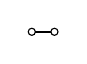
\begin{tikzpicture}[every node/.style={inner xsep=0pt,outer xsep=0pt}]%
\draw[fill = white] (0ex,.25ex) circle (.3ex);
\draw[thick] (.3ex,.25ex) -- (1.6ex,.25ex);%
\draw[fill = white] (1.9ex, .25ex) circle (.3ex);%
\end{tikzpicture}%
}
\newcommand{\latlinkna}{%
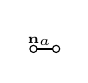
\begin{tikzpicture}[every node/.style={inner xsep=0pt,outer xsep=0pt}]
\node (A) at (0ex,1.0ex) {\tiny$\w{n}$};
\node (B) at (0.95ex,0.8ex) {\tiny$a$};
\draw[fill = white] (0ex,.25ex) circle (.3ex);
\draw[thick] (.3ex,.25ex) -- (1.6ex,.25ex);%
\draw[fill = white] (1.9ex, .25ex) circle (.3ex);%
\end{tikzpicture}%
}
\newcommand{\latlinkan}{%
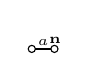
\begin{tikzpicture}[every node/.style={inner xsep=0pt,outer xsep=0pt}]
\node (A) at (1.95ex,1.0ex) {\tiny$\w{n}$};
\node (B) at (0.95ex,0.8ex) {\tiny$a$};
\draw[fill = white] (0ex,.25ex) circle (.3ex);
\draw[thick] (.3ex,.25ex) -- (1.6ex,.25ex);%
\draw[fill = white] (1.9ex, .25ex) circle (.3ex);%
\end{tikzpicture}%
}
\newcommand{\latlinknavec}{%
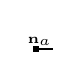
\begin{tikzpicture}[every node/.style={inner xsep=0pt,outer xsep=0pt}]
\node (A) at (0ex,1.0ex) {\tiny$\w{n}$};
\node (B) at (0.95ex,0.8ex) {\tiny$a$};
\draw[fill = black] (0ex,.06ex) rectangle ++(.4ex,.4ex);
\draw[thick] (.3ex,.25ex) -- (1.6ex,.25ex);%
\end{tikzpicture}%
}
\newcommand{\latlinkanvec}{%
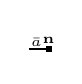
\begin{tikzpicture}[every node/.style={inner xsep=0pt,outer xsep=0pt}]
\node (A) at (1.95ex,1.0ex) {\tiny$\w{n}$};
\node (B) at (0.95ex,0.8ex) {\tiny$\bar{a}$};
\draw[thick] (.3ex,.25ex) -- (1.8ex,.25ex);%
\draw[fill = black] (1.8ex, .06ex) rectangle ++(.4ex,.4ex);%
\end{tikzpicture}%
}
\newcommand{\latlinkntvec}{%
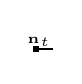
\begin{tikzpicture}[every node/.style={inner xsep=0pt,outer xsep=0pt}]
\node (A) at (0ex,1.0ex) {\tiny$\w{n}$};
\node (B) at (0.95ex,0.8ex) {\tiny$t$};
\draw[fill = black] (0ex,.06ex) rectangle ++(.4ex,.4ex);
\draw[thick] (.3ex,.25ex) -- (1.6ex,.25ex);%
\end{tikzpicture}%
}
\newcommand{\latlinknxvec}{%
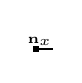
\begin{tikzpicture}[every node/.style={inner xsep=0pt,outer xsep=0pt}]
\node (A) at (0ex,1.0ex) {\tiny$\w{n}$};
\node (B) at (0.95ex,0.8ex) {\tiny$x$};
\draw[fill = black] (0ex,.06ex) rectangle ++(.4ex,.4ex);
\draw[thick] (.3ex,.25ex) -- (1.6ex,.25ex);%
\end{tikzpicture}%
}
%lattice square
%\newcommand{\latsquare}{%
%\begin{tikzpicture}[every node/.style={inner xsep=0pt,outer xsep=0pt}]%
%\draw[thick] (.3ex,.15ex) -- (1.6ex,.15ex);%
%\draw[thick] (1.87ex,.15ex) -- (1.87ex,1.45ex);%
%\draw[thick] (.3ex,1.75ex) -- (1.6ex,1.75ex);%
%\draw[thick] (0.03ex,.15ex) -- (0.03ex,1.45ex);%
%\draw[fill = white] (0ex,.15ex) circle (.3ex);
%\draw[fill = white] (1.9ex, .15ex) circle (.3ex);%
%\draw[fill = white] (1.9ex, 1.75ex) circle (.3ex);%
%\draw[fill = white] (0ex, 1.75ex) circle (.3ex);%
%\end{tikzpicture}%
%}
%\newcommand{\latsquarenab}{%
%\begin{tikzpicture}[every node/.style={inner xsep=0pt,outer xsep=0pt}]%
%\node (A) at (0ex,-0.5ex) {\tiny$\w{n}$};
%\node (B) at (1.05ex,-0.45ex) {\tiny$a$};
%\node (C) at (-0.4ex,0.9ex) {\tiny$b$};
%\draw[thick,decoration={markings,mark=at position 1 with {\arrow[scale=1,>=stealth]{>}}},postaction={decorate}] (.3ex,.15ex) -- (1.6ex,.15ex);%
%\draw[thick] (1.87ex,.15ex) -- (1.87ex,1.45ex);%
%\draw[thick] (.3ex,1.75ex) -- (1.6ex,1.75ex);%
%\draw[thick] (0.03ex,.15ex) -- (0.03ex,1.45ex);%
%\draw[fill = white] (0ex,.15ex) circle (.3ex);
%\draw[fill = white] (1.9ex, .15ex) circle (.3ex);%
%\draw[fill = white] (1.9ex, 1.75ex) circle (.3ex);%
%\draw[fill = white] (0ex, 1.75ex) circle (.3ex);%
%\end{tikzpicture}%
%}

\newcommand{\latsquare}{\ensuremath{%
  \mathchoice{\raisebox{-.5ex}{\includegraphics[height=2.3ex]{latsquare}}}
    {\raisebox{-.5ex}{\includegraphics[height=2.3ex]{latsquare}}}
    {\raisebox{-.5ex}{\includegraphics[height=1.8ex]{latsquare}}}
    {\raisebox{-.5ex}{\includegraphics[height=1.3ex]{latsquare}}}
}}
\newcommand{\latsquarenab}{\ensuremath{%
  \mathchoice{\raisebox{-.4ex}{\includegraphics[height=2.3ex]{latsquarenab}}}
    {\raisebox{-.4ex}{\includegraphics[height=2.3ex]{latsquarenab}}}
    {\raisebox{-.4ex}{\includegraphics[height=1.8ex]{latsquarenab}}}
    {\raisebox{-.4ex}{\includegraphics[height=1.3ex]{latsquarenab}}}
}}


%oleft (semidirect sum symbol)
\newcommand{\oleft}{%
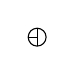
\begin{tikzpicture}[every node/.style={inner xsep=0pt,outer xsep=0pt}]
\draw[] (0ex,0ex) circle (.75ex);
\draw[] (-.75ex,0ex) -- (0ex,0ex);%
\draw[] (0ex,-.75ex) -- (0ex,.75ex);%
\end{tikzpicture}%
}

\newcommand{\blackcircle}{\raisebox{-.4ex}{\scalebox{1.66}{$\bullet$}}}
\newcommand{\whitedot}{\raisebox{.4ex}{\textcolor{white}{\scalebox{.3}{$\bullet$}}}}

%Gives \sfrac command to write 1/2 as a single character.
\usepackage{xfrac} 

%Discourages hyphenation!
%\usepackage[none]{hyphenat}

%Allows for \AsteriskRoundedEnds, and various stars, flowers, etc.
%http://texdoc.net/texmf-dist/doc/latex/comprehensive/symbols-a4.pdf
\usepackage{bbding}
%Allows \diamondplus
\DeclareFontFamily{U}{MnSymbolC}{}
\DeclareSymbolFont{MnSyC}{U}{MnSymbolC}{m}{n}
\DeclareMathSymbol{\diamondplus}{\mathbin}{MnSyC}{"7C}
\DeclareMathSymbol{\diamonddot}{\mathbin}{MnSyC}{"7E}
\DeclareFontShape{U}{MnSymbolC}{m}{n}{
    <-6>  MnSymbolC5
   <6-7>  MnSymbolC6
   <7-8>  MnSymbolC7
   <8-9>  MnSymbolC8
   <9-10> MnSymbolC9
  <10-12> MnSymbolC10
  <12->   MnSymbolC12}{}
  
  \newcommand\underlay[4]{%
  \stackengine{0pt}%
  {\kern#2\includegraphics[height=#1]{#4}}%
  {\includegraphics[height=#1]{#3}}%
  {O}{l}{F}{F}{L}%
}
\newcommand\addunderlay[4]{%
  \stackengine{0pt}%
  {\kern#2\includegraphics[height=#1]{#4}}%
  {#3}%
  {O}{l}{F}{F}{L}%
}

%EDIT: It would be nice to include hyperlinks but this package seems to have collisions with math mode.
\usepackage{hyperref}

%Multiple authors for IEEE format
%\usepackage{authblk}

%%%%%%%%%%%%%%%%%%%%%%%%%%%%%%%%%%%%%%%%%%%%%%%%%%%
%%%%%%%%%%%%%%%%%%%%%%%%%%%%%%%%%%%%%%%%%%%%%%%%%%%
%%%%%%%%%%%%%%%%%%%%%%%%%%%%%%%%%%%%%%%%%%%%%%%%%%%

% Use the \preprint command to place your local institutional report number 
% on the title page in preprint mode.
% Multiple \preprint commands are allowed.
%\preprint{.}

\begin{document}

\begin{frontmatter}

%\title{A scalable geometric generalization of Yee's method to unstructured meshes and higher order}
\title{Generalizing Yee's method: Scalable geometric higher-order\\FEEC algorithms for Maxwell's equations on an unstructured mesh}

%\title{Generalizing the Yee Algorithm to\\Unstructured Meshes and Higher Order} %Title of paper

\author[1]{Alexander S. Glasser}
\author[1,2]{Hong Qin}

\affiliation[1]{Princeton Plasma Physics Laboratory, Princeton University, Princeton, New Jersey 08543}
\affiliation[2]{Department of Astrophysical Sciences, Princeton University, Princeton, New Jersey 08544}
%\date{\today}

%\maketitle %\maketitle must follow title, authors, abstract and \pacs

%\hyphenpenalty=1000
\begin{abstract}
The Yee algorithm for electromagnetic simulations is widely known to have many advantages, including the following crucial two: (i) Its calculations are local and therefore efficiently parallelizable---enabling simulations that capitalize on the speed and scalability of high-performance computing architecture. \linebreak (ii) Yee's method faithfully preserves the symplectic geometry of Maxwell's equations, improving its accuracy in long-time numerical simulations. Whereas previous geometric generalizations of Yee's method have sacrificed its scalability, in this article the Yee algorithm is generalized to higher order and unstructured meshes in a manner that fully preserves both its scalability and geometric naturalness. This generalization is achieved by prioritizing the locality of the algorithm, reflecting the physical locality of Maxwell's equations. Specifically, we demonstrate that Yee's method is but a special case of a larger family of symplectic, finite element exterior calculus (FEEC) methods that use scalable, local approximations of mass matrices. We discuss the numerical advantages of this family of methods, which we call \emph{scalable FEEC} (SFEEC) methods.
\end{abstract}
%\hyphenpenalty=50
%\hyphenpenalty=1000

\end{frontmatter}

\section{Introduction}

\cmmnt{
A Hamiltonian formulation of Maxwell's equations

Maxwell's equations in vacuum can be compactly expressed in the notation of differential forms as
\begin{eqn}
\md F=0\hspace{36pt}\md\star F=0.
\end{eqn}
Here, ${F=\md A}$ denotes the electromagnetic tensor, a $\text{2-form}$ defined in flat $\mR^4$ spacetime in terms of the electromagnetic four-potential ${A^\alpha=(\phi,\w{A})}$ such that
\begin{eqn}
F&=\frac{1}{2}F_{\mu\nu}\md x^\mu\wedge\md x^\nu=\w{E}\\
\md A&=\md\big(A_\alpha\md x^\alpha\big)\\
&=\partial_t
\end{eqn}
}

The Yee algorithm \cite{yee_numerical_1966,taflove_computational_2005}---alternatively, the finite difference time domain (FDTD) method---defines electromagnetic fields on a cubic mesh. It associates to each edge a component of the electric field $\w{E}$, and to each face a component of the magnetic field $\w{B}$. This discretization reflects a natural geometric description of Maxwell's equations, in which one defines ${\w{E}\in\Lambda^1(\mR^3)}$ as a differential $\text{1-form}$ on $\mR^3$ and ${\w{B}\in\Lambda^2(\mR^3)}$ as a differential $\text{2-form}$ on $\mR^3$. In this way, Yee's method employs a technique adopted in many \emph{structure-preserving algorithms} \cite{hairer_geometric_2006}, wherein differential $k$-forms are discretized by associating them with $k$-dimensional features of a mesh \cite{whitney_geometric_1957,desbrun_discrete_2005,arnold_finite_2006,arnold_finite_2010}.

Structure-preserving algorithms have been widely adopted in many subfields of computational physics, including gravitational simulations  \cite{kinoshita_symplectic_1991,gladman_symplectic_1991,chambers_symplectic_2002,bravetti_numerical_2020,kur_discrete_2022}, geophysics \cite{li_structure-preserving_2012,liu_modified_2015} and plasma physics \cite{squire_geometric_2012,xiao_explicit_2015,he_hamiltonian_2015,crouseilles2015Hamiltonian,qin_canonical_2016,kraus_gempic:_2017,morrison_structure_2017,glasser_geometric_2020,glasser_gauge-compatible_2022}. Such algorithms generally derive from variational principles or Hamiltonian systems. As a result, they preserve essential mathematical features of their underlying physical systems, including symplectic structure, topology, symmetries, and conservation laws. These properties contribute to the numerical fidelity of structure-preserving algorithms, especially in long-time numerical simulations. Despite Yee's omission of any overt Lagrangian or Hamiltonian formulations in his original work \cite{yee_numerical_1966}, Yee's method (apparently serendipitously) is one of the most historically successful examples of a structure-preserving algorithm \cite{stern_geometric_2009}.

More recently, the methodology of structure-preserving algorithms has led to the development of advanced algorithms for the simulation of plasmas, whose electromagnetic fields are constructed using the formalism of finite element exterior calculus (FEEC) \cite{arnold_finite_2006,arnold_finite_2010,kraus_gempic:_2017,glasser_gauge-compatible_2022}. Although such methods are in principle readily generalizable to unstructured meshes and high order finite elements, they lack the computational efficiency and scalability of Yee's method. In particular, the time evolution of electromagnetic fields in these FEEC methods requires communication between all nodes of a simulation, thereby destroying their parallelism. As we shall discuss and address, this problem arises because sparse finite element mass matrices generally have dense inverses.

On the other hand, there have also been numerous efforts (e.g. \cite{bo_he_sparse_2006,he_differential_2007,kim_parallel_2011,teixeira_differential_2013}) to generalize Yee's method using scalable finite element methods, called finite element time domain (FETD) methods. Such efforts leverage the crucial technique of sparse approximate inverse (SPAI) mass matrices, and preserve the scalability of Yee's method. However, these methods' preservation of symplectic structure has not been established.

Motivated by the desire to overcome the scalability limitation of structure-preserving FEEC plasma methods, and to guarantee the structure preservation of FETD methods, in this article we develop \emph{scalable FEEC} (SFEEC) methods, a family of symplectic finite element methods for electromagnetic fields that includes Yee's method as a special case. SFEEC methods enable the higher order simulation of electromagnetic fields on structured and unstructured meshes in a manner that preserves the two aforementioned crucial advantages of Yee's method, namely: (i) its scalability on modern architectures; and (ii) its symplectic geometry (and the resulting conservation of electric charge and Gauss' law).

From a finite element point of view, the scalability of Yee's method will be reframed as a result of its simplified (or `pruned') approximation of finite element mass matrices. To retain their scalability, SFEEC methods employ a comparable, if more flexible treatment of mass matrices. Relative to Yee's method, SFFEC methods afford a greater flexibility to improve algorithmic accuracy without sacrificing scalability. Their use of finite elements and the FEEC formalism further enables their viability on more general meshes.

While Yee's algorithm has been generalized numerous times in the literature, including via higher order and finite element schemes (e.g. \cite{stern_geometric_2009,bo_he_sparse_2006,kim_parallel_2011,teixeira_differential_2013,hano_generalized_1997,cole_high-accuracy_1997,chen_generalization_2006,teixeira_time-domain_2008}), no such generalization is known to us that simultaneously affords higher order accuracy and scalability while ensuring the geometric structure-preservation of Yee's method. In particular, the Yee method's preservation of symplectic structure is an important aspect of the method's stability and long-term accuracy \cite{stern_geometric_2015}. In this work, we will review this symplectic structure of Yee's method and demonstrate its exact preservation in the SFEEC family of algorithms we define. In so doing, we also offer a means to overcome the scalability limitations of structure-preserving FEEC algorithms (e.g. \cite{kraus_gempic:_2017,glasser_gauge-compatible_2022}) in a massively parallel, high-performance computing architecture.

The remainder of this article is organized as follows. In Section~\ref{FEECsect}, the formalism of finite element exterior calculus (FEEC) \cite{arnold_finite_2006,arnold_finite_2010} and its discretization of electromagnetic fields will be reviewed. In Section~\ref{YeeIsFEEC}, it will be demonstrated that Yee's algorithm can be interpreted as an FEEC method with simplified mass matrices. In Section~\ref{GenYeeAlgos} we will define SFEEC methods, which extend Yee's method to higher order finite element schemes on a general mesh. In Section~\ref{NumResult}, numerical results will be presented that demonstrate the improved higher order accuracy of the resulting SFEEC methods relative to Yee's method, without sacrificing its scalability. Section~\ref{ConclusionSect} will then summarize and conclude.

\section{Finite Element Exterior Calculus (FEEC)\\for Electromagnetic Simulations\label{FEECsect}}

In this section, we briefly review aspects of FEEC \cite{arnold_finite_2006,arnold_finite_2010} and its application in electromagnetic simulations. We refer the reader to \cite{kraus_gempic:_2017,glasser_gauge-compatible_2022} for additional background. We let $\Lambda^p(\mT_h)$ denote a vector space of finite element differential $p\text{-form}$s on a simplicial or cubical complex ${\mT_h\subset\mR^n}$ (where the subscript $h$ denotes the maximal diameter, or edge length, of any simplex in $\mT_h$). For all ${0\leq p\leq n}$, $\Lambda^p(\mT_h)$ may be defined as the span of a finite ($N_p$-dimensional) basis ${\gv{\Lambda}^p}$, whose $i^\text{th}$ basis element ${\Lambda^p_i\in\Lambda^p(\mT_h)}$ is a piecewise polynomial $p\text{-form}$ on $\mT_h$. Such a basis element typically has support localized to one or more adjacent cells in ${\mT_h}$. An arbitrary $p\text{-form}$ ${\w{S}\in\Lambda^p(\mT_h)}$ can be expressed in the $\gv{\Lambda}^p$ basis as
\begin{eqn}
\w{S}(\w{x})&=\w{s}\cdot\gv{\Lambda}^p(\w{x})=s_i\Lambda^p_i(\w{x})
\label{basisElement}
\end{eqn}
$\forall$ ${\w{s}\in\mR^{N_p}}$ and ${\w{x}\in\abs{\mT_h}}$, the convex hull of ${\mT_h}$. (Einstein summation convention is used for the repeated index in Eq.~(\ref{basisElement}) and hereafter.) Individual components of ${\w{S}\in\Lambda^p(\mT_h)}$ will be denoted
\begin{eqn}
\w{S}(\w{x})_{\mu_1\cdots\mu_p}&=\w{s}\cdot\gv{\Lambda}^p(\w{x})_{\mu_1\cdots\mu_p}=s_i\Lambda^p_i(\w{x})_{\mu_1\cdots\mu_p}
\label{componentsOfForm}
\end{eqn}
where Greek letters denote coordinate indices. For example, given ${\abs{\mT_h}\subset\mR^3}$, the $\mu^\text{th}$ component of the $\text{1-form}$ basis element $\Lambda^1_i(\w{x})$ may be written as ${\Lambda^1_i(\w{x})_\mu}$ $\forall$ ${\mu\in\{1,2,3\}}$, such that ${\Lambda^1_i(\w{x})=\Lambda^1_i(\w{x})_\mu\md x^\mu}$.

Because each basis ${\gv{\Lambda}^p}$ is finite $\forall$ ${0\leq p\leq n}$, the exterior derivative ${\md:\Lambda^p(\mT_h)\rightarrow\Lambda^{p+1}(\mT_h)}$ of a finite element $p\text{-form}$ on ${\mT_h}$ can be computed in the ${\gv{\Lambda}^0,\dots,\gv{\Lambda}^n}$ bases by straightforward matrix multiplication. A choice of basis for each ${\Lambda^p(\mT_h)}$ in three dimensions (${\mT_h\subset\mR^3}$) determines, for example, matrices that represent the gradient ($\mG$), curl ($\mC$), and divergence ($\mathbb{D}$)---as defined in Table~\ref{dMatrixOps}.

\begin{table}[b!]
\setlength\tabcolsep{-0.5pt}
\renewcommand{\arraystretch}{1.3}
\centering
\hskip-0.25cm\begin{tabular*}{\columnwidth}{cccc}
\hline
~~~$p$-Form~~~ & ~~~Abstract $\md$~~~ & ~~~Matrix $\md$~~~ & ~Defined by~~\\
\hline
$\w{S}=\w{s}\cdot\gv{\Lambda}^0$ & - & - & -\\
\hline
$\w{A}=\w{a}\cdot\gv{\Lambda}^1$ & $\w{A}=\md\w{S}$ & $\w{a}=\mG\w{s}$ & $\mG^T\gv{\Lambda}^1=\md\gv{\Lambda}^0$\\
\hline
$\w{B}=\w{b}\cdot\gv{\Lambda}^2$ & $\w{B}=\md\w{A}$ & $\w{b}=\mC\w{a}$ & $\mC^T\gv{\Lambda}^2=\md\gv{\Lambda}^1$\\
\hline
$\w{C}=\w{c}\cdot\gv{\Lambda}^3$ & $\w{C}=\md\w{B}$ & ${\w{c}=\mmD\w{b}}$ & ${\mmD^T\gv{\Lambda}^3=\md\gv{\Lambda}^2}$\\
\hline
\end{tabular*}
\caption{FEEC matrix implementation of $\md$ on ${\mT_h\subset\mR^3}$. The property ${\md\circ\md=0}$ implies that ${\mC\mG=\mZero}$ and ${\mmD\mC=\mZero}$.}
\label{dMatrixOps}
\end{table}

To apply FEEC in a physical setting, it will also be essential to compute \emph{mass matrices} on $\mT_h$ for each basis $\gv{\Lambda}^p$ of finite element $p\text{-form}$s. Specifically, the mass matrix ${\mM_p\in\mR^{N_p\times N_p}}$ for $\gv{\Lambda}^p$ is defined by
\begin{eqn}
(\mM_p)_{ij}&=\int_{\abs{\mT_h}}\hspace{-3pt}\md\w{x}\Big(\Lambda^p_i,\Lambda^p_j\Big)_p
\label{Mpdef}
\end{eqn}
where ${(\cdot,\cdot)_p}$ denotes the pointwise inner product on $p\text{-form}$s induced by the metric $g_{\mu\nu}$---specifically
\begin{eqn}
(\alpha,\beta)_p&=\frac{1}{p!}\alpha_{\mu_1\cdots\mu_p}\beta^{\mu_1\cdots\mu_p}\\
&=\frac{1}{p!}\alpha_{\mu_1\cdots\mu_p}\beta_{\nu_1\cdots\nu_p}g^{\mu_1\nu_1}\cdots g^{\mu_p\nu_p}.
\label{pFormInnerProd}
\end{eqn}
For ${p=1,2}$ on $\mR^3$, for example, Eq.~(\ref{pFormInnerProd}) defines the inner product ${(\alpha,\beta)_p}$ as the standard inner product ${\alpha\cdot\beta}$. After all, 1- and $\text{2-form}$s each have three independent components in $\mR^3$, and the metric ${g_{\mu\nu}}$ (and its inverse ${g^{\mu\nu}}$) is given by the Kronecker delta---${g_{\mu\nu}=\delta_{\mu\nu}}$. We note that ${(\alpha,\beta)_p}$ is symmetric, such that Eq.~(\ref{Mpdef}) is symmetric and ${\mM_p^T=\mM_p}$. Eq.~(\ref{Mpdef}) also implies that $\mM_p$ is typically sparse (so long as each basis element $\Lambda_i^p$ has only local support). Importantly, however, its inverse matrix $\mM_p^{-1}$ is typically dense.

To apply the FEEC formalism to electromagnetic simulations, we will first discretize the magnetic vector potential as an FEEC $\text{1-form}$, that is,
\begin{eqn}
\w{A}=\w{a}\cdot\gv{\Lambda}^1
\end{eqn}
with degrees of freedom given by the vector of coefficients ${\w{a}\in\mR^{N_1}}$. (We work in the temporal gauge, such that the electric potential $\phi$ vanishes, ${\phi=0}$.) The magnetic field is then given by a $\text{2-form}$,
\begin{eqn}
\w{B}=\w{b}\cdot\gv{\Lambda}^2=\mC\w{a}\cdot\gv{\Lambda}^2=\w{a}\cdot\mC^T\gv{\Lambda}^2=\w{a}\cdot\md\gv{\Lambda}^1=\md\w{A}
\end{eqn}
with ${\w{b}\in\mR^{N_2}}$, in keeping with the geometry of Maxwell's equations and the FEEC implementation of the curl, as in Table~\ref{dMatrixOps}. Lastly, the electric field will be defined as a discrete $\text{1-form}$
\begin{eqn}
\w{E}=\w{e}\cdot\mM_1^{-1}\cdot\gv{\Lambda}^1
\end{eqn}
with ${\w{e}\in\mR^{N_1}}$. Following \cite{glasser_gauge-compatible_2022}, we use a convention wherein the coefficients $\w{e}$ determine the electric field $\w{E}$ with an additional factor of $\mM_1^{-1}$. We shall regard the pair ${(\w{a},\w{e})\in\mR^{2N_1}}$ as defining the degrees of freedom of the electromagnetic finite element dynamical system.

To describe the dynamics of these discrete fields via Maxwell's equations, we first recall the canonical symplectic structure of electromagnetic fields in the continuum, defined with Poisson bracket and Hamiltonian in SI units as \cite{marsden_hamiltonian_1982}
\begin{eqn}
\{F,G\}_{\text{EM}}&=\frac{1}{\epsilon_0}\int\md\w{x}\left(\frac{\delta F}{\delta \w{E}}\cdot\frac{\delta G}{\delta \w{A}}-\frac{\delta G}{\delta \w{E}}\cdot\frac{\delta F}{\delta \w{A}}\right)\\
H_{\text{EM}}&=\frac{1}{2}\int\md\w{x}\left(\epsilon_0\abs{\w{E}}^2+\frac{1}{\mu_0}\abs{\nabla\times\w{A}}^2\right).
\label{continuumEMHamil}
\end{eqn}
We now substitute the FEEC fields ${\w{A}=\w{a}\cdot\gv{\Lambda}^1}$ and ${\w{E}=\w{e}\cdot\mM_1^{-1}\cdot\gv{\Lambda}^1}$ into Eq.~(\ref{continuumEMHamil}) to derive (see \cite{glasser_gauge-compatible_2022}) the following discrete Poisson bracket ${\{\cdot,\cdot\}_\Delta}$ and discrete Hamiltonian $H_\Delta$ approximating this system,
\begin{eqn}
\{F,G\}_\Delta&=\frac{1}{\epsilon_0}\left(\pd{F}{\w{e}}\cdot\pd{G}{\w{a}}-\pd{G}{\w{e}}\cdot\pd{F}{\w{a}}\right)\\
H_\Delta&=\frac{1}{2}\left(\epsilon_0\w{e}^T\mM_1^{-1}\w{e}+\frac{1}{\mu_0}\w{a}^T\mC^T\mM_2\mC\w{a}\right),
\label{discHamilSystem}
\end{eqn}
where we have applied ${\md\gv{\Lambda}^1=\mC^T\gv{\Lambda}^2}$ as in Table~\ref{dMatrixOps}.

Equations of motion are now readily calculated as usual with a Poisson bracket. We plug the FEEC coefficient vectors $\w{a}$ and $\w{e}$ into ${\{\cdot,\cdot\}_\Delta}$ with $H_\Delta$, to find
\begin{eqn}
\dot{\w{a}}&=\{\w{a},H_\Delta\}_\Delta=-\mM_1^{-1}\w{e}\\
\dot{\w{e}}&=\{\w{e},H_\Delta\}_\Delta=c^2\mC^T\mM_2\mC\w{a}.
\label{discEOM}
\end{eqn}
These equations are discrete forms of Maxwell's equations, ${\dot{\w{A}}=-\w{E}}$ and ${\dot{\w{E}}=c^2\nabla\times\nabla\times\w{A}}$, respectively. In Section \ref{NumResult}, the discrete approximation of the curl-of-curl operator
\begin{eqn}
\nabla\times\nabla\times\approx\mM_1^{-1}\mC^T\mM_2\mC,
\label{curlOfCurl}
\end{eqn}
whose calculation (until our later simplification) incorporates the dense matrix $\mM_1^{-1}$, will be a central focus of our study. 

Note, it will also be convenient to rewrite Eq.~(\ref{discEOM}) in terms of the magnetic field by substituting ${\w{b}=\mC\w{a}}$ (the discrete realization of ${\w{B}=\nabla\times\w{A}}$) to find
\begin{eqn}
\dot{\w{b}}&=-\mC\mM_1^{-1}\w{e}\\
\dot{\w{e}}&=c^2\mC^T\mM_2\w{b}.
\label{preYeeFEECEqns}
\end{eqn}
Because of the gauge symmetry of Maxwell's equations, Eq.~(\ref{preYeeFEECEqns}) is an equivalent formulation of Eq.~(\ref{discEOM}) and exactly preserves the physical degrees of freedom of interest \cite{glasser_geometric_2020,glasser_gauge-compatible_2022}.

To algorithmically evolve Eq.~(\ref{discEOM}) in discrete time, we follow \cite{he_hamiltonian_2015} (see also \cite{glasser_geometric_2020}) and define a splitting algorithm that decomposes $H_\Delta$ of Eq.~(\ref{discHamilSystem}) into two pieces:
\begin{eqn}
H_\Delta&=H_\w{a}+H_\w{e}\\
\text{where}~~~H_\w{a}&=\frac{1}{2\mu_0}\w{a}^T\mC^T\mM_2\mC\w{a}\\
H_\w{e}&=\frac{\epsilon_0}{2}\w{e}^T\mM_1^{-1}\w{e}.
\end{eqn}
These `sub-Hamiltonians' define two different subsystems which may be evolved separately, that is,
\begin{eqn}
H_\w{a}&
\begin{cases}
\dot{\w{a}}&=\{\w{a},H_\w{a}\}_\Delta=0\\
\dot{\w{e}}&=\{\w{e},H_\w{a}\}_\Delta=c^2\mC^T\mM_2\mC\w{a}.
\end{cases}\\
H_\w{e}&
\begin{cases}
\dot{\w{a}}&=\{\w{a},H_\w{e}\}_\Delta=-\mM_1^{-1}\w{e}\\
\dot{\w{e}}&=\{\w{e},H_\w{e}\}_\Delta=0.
\end{cases}
\label{subsystemEvolutions}
\end{eqn}
We see that $\w{a}$ is constant in the subsystem $H_\w{a}$, while $\w{e}$ is constant in the subsystem $H_\w{e}$. As a result, each subsystem is exactly solvable over a finite time interval $\Delta t$, in particular,
\begin{eqn}
H_\w{a}:~~~~\w{e}(t_0+\Delta t)&=\w{e}(t_0)+\Delta t\cdot c^2\mC^T\mM_2\mC\w{a}(t_0)\\
H_\w{e}:~~~~\w{a}(t_0+\Delta t)&=\w{a}(t_0)-\Delta t\cdot\mM_1^{-1}\w{e}(t_0).
\label{subsysEvolutions}
\end{eqn}
By choosing an appropriate sequence of these subsystems' discrete time evolutions, a splitting method may be implemented that approximates a timestep of the entire electromagnetic system $H_\Delta$.

A typical example of such a splitting scheme is called Strang splitting \cite{strang_construction_1968}, which evolves $\w{a}$ and $\w{e}$ according to the approximation
\begin{eqn}
\left[\begin{matrix}\w{a}\\\w{e}\end{matrix}\right]_{\mathrlap{t_0+\Delta t}}&~~~=\exp\left(\Delta tH_\Delta\right)\cdot\left[\begin{matrix}\w{a}\\\w{e}\end{matrix}\right]_{t_0}\\
&\approx\exp\left(\frac{\Delta t}{2}H_\w{e}\right)\exp\left(\Delta tH_\w{a}\right)\exp\left(\frac{\Delta t}{2}H_\w{e}\right)\cdot\left[\begin{matrix}\w{a}\\\w{e}\end{matrix}\right]_{t_0}.
\label{splitEvolution}
\end{eqn}
Here, we use the notation ${\exp(\Delta tH_i)}$ to denote a discrete time mapping---as appears in Eq.~(\ref{subsysEvolutions})---that evolves according to the Hamiltonian $H_i$ for a time interval $\Delta t$. Since $\exp(\Delta tH_\w{a})$ and $\exp(\Delta tH_\w{e})$ do not commute, the second line of Eq.~(\ref{splitEvolution}) is only an approximation of the first. Nevertheless, such a splitting method is an effective algorithmic implementation of our dynamical system. It is exactly solvable, accurate to second order, and preserves the symplectic structure of the system as defined by the Poisson bracket of Eq.~(\ref{discHamilSystem}). Splitting methods of arbitrarily high accuracy in $\Delta t$ can also be constructed (see, e.g. \cite{hairer_geometric_2006}).

\section{Reinterpreting Yee's Method via FEEC\label{YeeIsFEEC}}

We now rederive Yee's method using the finite element formalism of the previous section. We proceed in three steps: (i) we first choose generalized Whitney forms as an FEEC basis on a cubical mesh; (ii) we then maximally simplify the mass matrices of the corresponding electromagnetic algorithm; and finally (iii) we choose Strang splitting as our method of time evolution. These three steps will exactly recover Yee's method, demonstrating its interpretation as an implementation of the FEEC electromagnetic algorithm defined in Eq.~(\ref{subsysEvolutions})---with simplified mass matrices.

We begin by considering a cubical lattice ${\mT_h\subset\mR^3}$ with lattice spacings ${\{\Delta_x,\Delta_y,\Delta_z\}}$. We make the simplest possible choice for an FEEC basis on $\mT_h$, namely, the \emph{generalized Whitney forms}, a family of piecewise polynomial finite elements denoted ${Q_1^-\Lambda^p(\mT_h)}$ \cite{arnold_periodic_nodate}). This finite element basis is also usefully defined in \cite{lohi_whitney_2021} Example~5.2.

A generalized Whitney $p\text{-form}$ can be readily understood by its 1-to-1 correspondence with a $p$-dimensional feature of a mesh. In particular, we define the generalized Whitney $p\text{-form}$ ${\mW_{\sigma^p}\in Q_1^-\Lambda^p(\mT_h)}$ associated to a given $p$-face ${\sigma^p\subset\mT_h\subset\mR^n}$ by requiring that
\begin{eqn}
\frac{1}{\abs{\tau^p}}\int_{\tau^p}\mW_{\sigma^p} =
\begin{cases}
1 & \tau^p=\sigma^p\\
0&\tau^p\neq\sigma^p.
\end{cases}
\label{WhitneyFormDefn}
\end{eqn}
In this way, generalized Whitney $p\text{-form}$s are \emph{dual} to $p$-faces of $\mT_h$ via integration. Here, ${\abs{\tau^p}}$ denotes the $p$-volume of $\tau^p$ (defined as 1, length, area, and volume respectively for ${p=0,1,2,3}$). This normalization is chosen to mimic fields as they are typically represented in Yee's method.

A concrete example of this is represented on ${\mT_h\subset\mR^3}$ in Fig.~\ref{GenWhitneyCubes}. The $\text{1-form}$ ${\mW_{x_1x_2}\in Q_1^-\Lambda^1(\mT_h)}$ and the $\text{2-form}$ ${\mW_{x_1x_2x_4x_3}\in Q_1^-\Lambda^2(\mT_h)}$ are depicted, defined respectively by
\begin{eqn}
\mW_{x_1x_2}&=\left(1-\tfrac{y}{\Delta_y}\right)\left(1-\tfrac{z}{\Delta_z}\right)\md x\\
\mW_{x_1x_2x_4x_3}&=\left(1-\tfrac{z}{\Delta_z}\right)\md x\wedge\md y.
\label{whitneyEx12}
\end{eqn}
As in Eq.~(\ref{WhitneyFormDefn}), $\mW_{x_1x_2}$ is the least-order piecewise polynomial $\text{1-form}$ satisfying ${\int_{x_1x_2}\mW_{x_1x_2}=\abs{x_1x_2}}$ and ${\int_{\sigma^1}\mW_{x_1x_2}=0}$ $\forall$ ${\sigma^1\neq x_1x_2}$. $\mW_{x_1x_2x_4x_3}$ is analogously defined so that its integral satisfies ${\int_{x_1x_2x_4x_3}\mW_{x_1x_2x_4x_3}=\abs{x_1x_2x_4x_3}}$ and vanishes on any other face. In later calculations, it will also be useful to explicitly define the following Whitney $\text{2-form}$ associated to the face ${x_1x_5x_6x_2}$ in Fig.~\ref{GenWhitneyCubes},
\begin{eqn}
\mW_{x_1x_5x_6x_2}&=\left(1-\tfrac{y}{\Delta_y}\right)\md z\wedge\md x.
\label{whitneyEx12_a}
\end{eqn}

\begin{figure}[b!]
\centering
\underlay{1.5in}{120pt}{1formsWhitney.png}{2formsWhitney.png}
\caption{The generalized Whitney $\text{1-form}$s $\mW_{x_1x_2}$ and $\mW_{x_1x_2x_4x_3}$ are schematically depicted, respectively, on the left and right. $\mW_{x_1x_2}$ evaluates to the length $\abs{x_1x_2}$ when integrated along the edge ${x_1x_2}$ (in blue) and vanishes on all other edges (in orange). $\mW_{x_1x_2x_4x_3}$ likewise yields the area $\abs{x_1x_2x_4x_3}$ when integrated over the blue face ${x_1x_2x_4x_3}$, and vanishes on all other faces.}
\label{GenWhitneyCubes}
\end{figure}

Now consider the exterior derivative $\md$ of these forms. The curl matrix ${\mC:\mR^{N_1}\rightarrow\mR^{N_2}}$ is a linear operator that precisely computes $\md$ for $\text{1-form}$s, mapping the coefficients of a discrete $\text{1-form}$---expanded in the ${Q_1^-\Lambda^1(\mT_h)}$ basis---to coefficients of a discrete $\text{2-form}$---expanded in the ${Q_1^-\Lambda^2(\mT_h)}$ basis. The ${\text{1-to-1}}$ correspondence between these generalized Whitney forms and elements of the mesh leads to a convenient interpretation of $\mC$ in that basis, as follows.

We find by directly computing the exterior derivative of $\mW_{x_1x_2}$ using Eqs.~(\ref{whitneyEx12}-\ref{whitneyEx12_a}), for example, that
\begin{eqn}
\md\mW_{x_1x_2}&=\frac{1}{\Delta_y}\mW_{x_1x_2x_4x_3}-\frac{1}{\Delta_z}\mW_{x_1x_5x_6x_2}.
\label{dCurlExample}
\end{eqn}
We observe that a Whitney $\text{2-form}$ $\mW_{\sigma^2}$ appears on the right hand side above if and only if its associated face $\sigma^2$ contains the edge $x_1x_2$ on its boundary. Its coefficient ${\pm1/\Delta_{x^\mu}}$ is determined by the $\mu^{\text{th}}$ dimension in which the associated face extends $x_1x_2$, and its sign is set by the relative orientation between the edge and face.

Note, this interpretation of $\md$---as a mapping with coefficients ${\pm1/\Delta_{x^\mu}}$ from $\text{1-form}$s to the $\text{2-form}$s of faces which contain them on the boundary---is applicable only to the particular (cubical) FEEC mesh and (Whitney form) FEEC basis that we have chosen. In this context, however, our interpretation leads us to note that the curl operator $\mC$, (which implements $\md$ as defined in Table~\ref{dMatrixOps}), acts on on the generalized Whitney forms of a cubical lattice as nothing more than a finite difference operator. To see this more explicitly, let us denote by ${\w{a}_{\sigma^1}}$ the entry of ${\w{a}\in\mR^{N_1}}$ corresponding to the Whitney $\text{1-form}$ basis element ${\mW_{\sigma^1}}$. Likewise, we let ${\w{b}_{\sigma^2}}$ denote the coefficient in  ${\w{b}=\mC\w{a}\in\mR^{N_2}}$ corresponding to ${\mW_{\sigma^2}}$. With reference again to Fig.~\ref{GenWhitneyCubes}, we find that
\begin{eqn}
\w{b}_{x_1x_2x_4x_3}&=(\mC\w{a})_{x_1x_2x_4x_3}\\
&=\frac{1}{\Delta_x}\Big(\w{a}_{x_2x_4}-\w{a}_{x_1x_3}\Big)-\frac{1}{\Delta_y}\Big(\w{a}_{x_3x_4}-\w{a}_{x_1x_2}\Big).
\label{dIsFiniteDiff}
\end{eqn}
Under the map $\mC$, the finite differences of the edge coefficients are therefore summed to derive the coefficient on a face.

The transpose of the curl operator $\mC^T$, yields an analogous result, with ${(\mC^T\w{b})_{\sigma^1}}$ computed via finite differences between the faces adjoining edge $\sigma^1$. Using Fig.~\ref{CTranspGraphic} as a reference, for example, we find
\begin{eqn}
(\mC^T\w{b})_{x_1x_5}=\frac{1}{\Delta_x}\Big(\w{b}&_{x_1x_5x_6x_2}-\w{b}_{x_{10}x_{12}x_5x_1}\Big)\\
&-\frac{1}{\Delta_y}\Big(\w{b}_{x_1x_3x_7x_5}-\w{b}_{x_{9}x_{1}x_5x_{11}}\Big).
\label{dTIsFiniteDiff}
\end{eqn}

\begin{figure}[t!]
\includegraphics[width=\linewidth]{CTranspGraphic.png}
\caption{A depiction of the degrees of freedom involved in $\mC^T$---the transposed curl operator---for generalized Whitney forms on a cubic mesh.}
\label{CTranspGraphic}
\end{figure}

The observation that $\mC$ acts as a finite difference operator on cubical generalized Whitney forms marks a first step toward recovering Yee's method from Eq.~(\ref{subsysEvolutions}).

As a second step, let us first consider what $\mM_1$ and $\mM_2$ look like for our chosen Whitney form FEEC basis on a cubical mesh. Ignoring boundary cells for simplicity, we use Eq.~(\ref{Mpdef}) to integrate inner products of forms such as those appearing in Eq.~(\ref{whitneyEx12}) to find that
\begin{eqn}
(\mM_1)_{\sigma^1,\tau^1}&=\Delta_V\cdot
\begin{cases}
4/9&\sigma^1=\tau^1\\
1/9&\sigma^1\parallel\tau^1\text{ and }\exists~\tau^2\supset\{\sigma^1,\tau^1\}\\
1/36&\sigma^1\parallel\tau^1\text{ and }\exists~\tau^3\supset\{\sigma^1,\tau^1\}
\end{cases}\\
(\mM_2)_{\sigma^2,\tau^2}&=\Delta_V\cdot
\begin{cases}
2/3&\sigma^2=\tau^2\\
1/6&\sigma^2\parallel\tau^2\text{ and }\exists~\tau^3\supset\{\sigma^2,\tau^2\}
\end{cases}
\label{whitMassMatrices}
\end{eqn}
where ${\Delta_V=\Delta_x\Delta_y\Delta_z}$ denotes a cell volume. Given these matrix entries, each row (and column) of $\mM_1$ and $\mM_2$ can be readily shown to sum to $\Delta_V$. In the interest of recovering Yee's method, therefore, we define the simplified mass matrices
\begin{eqn}
\mM_1^Y&=\Delta_V\cdot\mOne_{N_1\times N_1}\\
\mM_2^Y&=\Delta_V\cdot\mOne_{N_2\times N_2}.
\label{YeeMassMatrices}
\end{eqn}
Here, $\mM_p^Y$ signifies the `Yee-modified' mass matrix for $p\text{-form}$s, and $\mOne$ denotes the identity matrix. This process is often referred to as `lumping' the mass matrix (of Eq.~(\ref{whitMassMatrices}), for example) into diagonal form.

Importantly, using such simplified mass matrices leaves the symplectic structure defined by ${\{\cdot,\cdot\}_\Delta}$ in Eq.~(\ref{discHamilSystem}) entirely undisturbed. Rather, a substitution of the simplified mass matrix ${\mM_p\rightarrow\mM_p^Y}$ is properly viewed as taking place within the discrete Hamiltonian $H_\Delta$ in Eq.~(\ref{discHamilSystem}). While this coarser approximation of $H_{\text{EM}}$ reduces the accuracy of the resulting (Yee's) algorithm, it has no deleterious effect on its characterization as a structure-preserving algorithm.

We now complete our program to recover Yee's method. Let us consider again the Strang splitting defined in Eq.~(\ref{splitEvolution}). We can rewrite this system more explicitly as
\begin{eqn}
\left[\begin{matrix}\w{a}\\\w{e}\end{matrix}\right]_{\mathrlap{t_0+\Delta t}}~~&=~~\mH_\w{e}^{\Delta t/2}\mH_\w{a}^{\Delta t}\mH_\w{e}^{\Delta t/2}\left[\begin{matrix}\w{a}\\\w{e}\end{matrix}\right]_{t_0}~~~\text{where}\\
\mH_\w{e}^{\Delta t}&=\left[\begin{matrix}\mOne&-\Delta t\mM_1^{-1}\\\mZero&\mOne\end{matrix}\right]~~\text{,}~~\mH_\w{a}^{\Delta t}=\left[\begin{matrix}\mOne&\mZero\\\Delta tc^2\mC^T\mM_2\mC&\mOne\end{matrix}\right]
\label{explicitEASplit}
\end{eqn}
or equivalently, in terms of ${\w{b}=\mC\w{a}}$:
\begin{eqn}
\left[\begin{matrix}\w{b}\\\w{e}\end{matrix}\right]_{\mathrlap{t_0+\Delta t}}&~~=~~\mmH_\w{e}^{\Delta t/2}\mmH_\w{b}^{\Delta t}\mmH_\w{e}^{\Delta t/2}\left[\begin{matrix}\w{b}\\\w{e}\end{matrix}\right]_{t_0}~~~\text{where}\\
\mmH_\w{e}^{\Delta t}&=\left[\begin{matrix}\mOne&-\Delta t\mC\mM_1^{-1}\\\mZero&\mOne\end{matrix}\right]~~~\text{,}~~~\mmH_\w{b}^{\Delta t}=\left[\begin{matrix}\mOne&\mZero\\\Delta tc^2\mC^T\mM_2&\mOne\end{matrix}\right].
\label{explicitEBSplit}
\end{eqn}
Eq.~(\ref{explicitEBSplit}) is iterated in a simulation, so that after ${n+1}$ timesteps its evolution operator is ${\mmH_\w{e}^{\Delta t/2}\left[\mmH_\w{e}^{\Delta t}\mmH_\w{b}^{\Delta t}\right]^n\mmH_\w{e}^{\Delta t/2}}$. Therefore, applying the `finite-difference operators' $\mC$ and $\mC^T$ from Eqs.~(\ref{dIsFiniteDiff}-\ref{dTIsFiniteDiff}) and the mass matrix approximations $\mM_p^Y$ from Eq.~(\ref{YeeMassMatrices}), let us examine our splitting method at `mid-step'---after ${[\mmH_\w{e}^{\Delta t}\mmH_\w{b}^{\Delta t}]\mmH_\w{e}^{\Delta t/2}}$---and compare it with Yee's method.

Since ${\mmH_\w{e}^{\Delta t/2}}$ only evolves $\w{b}$, we regard this as an `initialization step' that gives us
\begin{eqn}
\mmH_\w{e}^{\Delta t/2}:\left(\begin{matrix}\w{b}[t_0]\\\w{e}[t_0]\end{matrix}\right)\mapsto\left(\begin{matrix}\w{b}\left[t_{1/2}\right]\\\w{e}\left[t_0\right]\end{matrix}\right).
\end{eqn}
In particular, this half-step establishes initial field data as it appears in Yee's method. Next, ${\mmH_\w{b}^{\Delta t}}$ only evolves $\w{e}$, such that
\begin{eqn}
\mmH_\w{b}^{\Delta t}:\left(\begin{matrix}\w{b}\left[t_{1/2}\right]\\\w{e}\left[t_0\right]\end{matrix}\right)\mapsto\left(\begin{matrix}\w{b}\left[t_{1/2}\right]\\\w{e}\left[t_1\right]\end{matrix}\right)\\[0.5em]
\text{ where }\w{e}\left[t_1\right]=\w{e}\left[t_0\right]+\Delta t\Delta_Vc^2\mC^T\w{b}[t_{1/2}].
\label{YeeRecover1}
\end{eqn}
This timestep ${(\w{e}\left[t_1\right]-\w{e}\left[t_0\right])/\Delta tc^2=\Delta_V\mC^T\w{b}[t_{1/2}]}$ replicates the Yee method's evolution of the electric field, e.g.
\begin{eqn}
&\frac{1}{c^2 \Delta t}\left(E_x^{n+1}\left[i+\tfrac{1}{2},j,k\right]-E_x^n\left[i+\tfrac{1}{2},j,k\right]\right)\\
&=\frac{1}{\Delta y}\left(B_z^{n+\frac{1}{2}}\left[i+\tfrac{1}{2},j+\tfrac{1}{2},k\right]-B_z^{n+\frac{1}{2}}\left[i+\tfrac{1}{2},j-\tfrac{1}{2},k\right]\right)\\
&-\frac{1}{\Delta z}\left(B_y^{n+\frac{1}{2}}\left[i+\tfrac{1}{2},j,k+\tfrac{1}{2}\right]-B_y^{n+\frac{1}{2}}\left[i+\tfrac{1}{2},j,k-\tfrac{1}{2}\right]\right).
\label{Yee1}
\end{eqn}
As depicted in Fig.~\ref{CTranspGraphic} and described in Eq.~(\ref{dTIsFiniteDiff}), the operator $\mC^T$ implements precisely the finite differences of Eq.~(\ref{Yee1}). The additional constant factor $\Delta_V$ in Eq.~(\ref{YeeRecover1}) has no effect other than changing the effective unit in which $\w{b}$ is expressed. Finally, ${\mmH_\w{e}^{\Delta t}}$ only evolves $\w{b}$, such that
\begin{eqn}
\mmH_\w{e}^{\Delta t}:\left(\begin{matrix}\w{b}\left[t_{1/2}\right]\\\w{e}\left[t_1\right]\end{matrix}\right)\mapsto\left(\begin{matrix}\w{b}\left[t_{3/2}\right]\\\w{e}\left[t_1\right]\end{matrix}\right)\\[0.5em]
\text{ where }\w{b}\left[t_{3/2}\right]=\w{b}\left[t_{1/2}\right]-(\Delta t/\Delta_V)\mC\w{e}[t_{1}].
\label{YeeRecover2}
\end{eqn}
This timestep ${(\w{b}\left[t_{3/2}\right]-\w{b}\left[t_{1/2}\right])\Delta_V/\Delta t=\mC\w{e}[t_{1}]}$ replicates Yee's evolution of the magnetic field, e.g.
\begin{eqn}
\frac{1}{\Delta t}&\left(B_x^{n+\frac{1}{2}}\left[i,j+\tfrac{1}{2},k+\tfrac{1}{2}\right]-B_x^{n-\frac{1}{2}}\left[i,j+\tfrac{1}{2},k+\tfrac{1}{2}\right]\right)\\
&=\frac{1}{\Delta z}\left(E_y^n\left[i,j+\tfrac{1}{2},k+1\right]-E_y^n\left[i,j+\tfrac{1}{2},k\right]\right)\\
&-\frac{1}{\Delta y}\left(E_z^n\left[i,j+1,k+\tfrac{1}{2}\right]-E_z^n\left[i,j,k+\tfrac{1}{2}\right]\right).
\label{Yee2}
\end{eqn}
As described in Eq.~(\ref{dIsFiniteDiff}), $\mC$ implements precisely the finite differences of Eq.~(\ref{Yee2}). The factor of $\Delta_V$ again only impacts the unit of $\w{b}$.

Consequently, we have demonstrated that Yee's algorithm is equivalent to the structure-preserving FEEC method of Eq.~(\ref{subsysEvolutions}), using Whitney forms on a cubical mesh, maximally simplified (diagonal) mass matrices, and Strang splitting time evolution.

\section{Generalizing Yee's Method\label{GenYeeAlgos}}

\begin{table*}[t!]
%\setlength\tabcolsep{-0.5pt}
%\extracolsep{\fill}}
\renewcommand{\arraystretch}{1.1}
\centering
\begin{tabular*}{0.787\textwidth}{|c|c|c|}
\hline
 & \textbf{Yee's Method} & \textbf{SFEEC methods}\\
 \hline
Splitting method & Strang & any (e.g. Lie-Trotter \cite{trotter_product_1959}, Strang)\\
 \hline
Mesh & cubical & any (e.g. simplicial, cubical)\\
\hline
Finite elements & Whitney forms & any FEEC basis (e.g. ${\mmP_r^-\Lambda^k,\mmP_r\Lambda^k}$)\\
\hline
$\mM_1^{-1}$ and $\mM_2$  & diagonal approximation & any sparse approximation\\
\hline
\end{tabular*}
\caption{The SFEEC generalization of Yee's method affords considerable flexibility in the choice of splitting scheme, mesh, and finite element basis in its implementation of Eq.~(\ref{subsysEvolutions}). SFEEC methods are symplectic and are also required to be scalable. Therefore, they require sparse mass matrices and their sparse approximate inversions.}
\label{YeeVsSFEEC}
\end{table*}

The previous section demonstrates that Yee's method is a special case of the FEEC structure-preserving algorithm defined by Eq.~(\ref{subsysEvolutions}). Specifically, Yee's method is seen to make several selections for the FEEC algorithm, including
\begin{enumerate}
\item timesteps given by a Strang splitting scheme;
\item a cubical grid;
\item the least-order FEEC finite element basis---cubical Whitney forms; and
\item mass matrices simplified into diagonal form.
\end{enumerate}
The last of these---the mass matrix approximation---can be seen not so much as a `selection' but as a `departure' from the algorithm defined by Eq.~(\ref{subsysEvolutions}). As previously described, however, a simplified treatment of mass matrices occurs at the level of the Hamiltonian $H_\Delta$ in Eq.~(\ref{discHamilSystem}), and does not affect the Poisson bracket ${\{\cdot,\cdot\}_\Delta}$. As a result, Yee's method remains symplectic and---though it loses accuracy---retains all of the advantages of a structure-preserving algorithm. Yee's method thereby preserves the geometric structure of Maxwell's equations while employing a parsimonious description of electromagnetic fields. Moreover, its sacrifice of accuracy in mass matrices is arguably compensated by the scalability the Yee method achieves.

Here, we propose to relax all four of the above selections made for the Yee scheme, and in so doing we define a new class of algorithms, \emph{scalable FEEC} (SFEEC) methods. In particular, Table~\ref{YeeVsSFEEC} enumerates the generalizations of Yee's method afforded by SFEEC methods.

As defined, SFEEC methods offer considerable flexibility in generalizing the Yee scheme. They have the full flexibility of FEEC behind them, and can therefore handle quite general meshes and high order finite elements. Moreover, the splitting scheme used for SFEEC methods can be chosen to be of arbitrarily high order accuracy in time.

As we shall see, however, this improvement in accuracy is constrained by the requirement that SFEEC methods remain scalable. In particular, while mass matrices will no longer be maximally simplified into diagonal form (as in Yee's approach), $\mM_1^{-1}$ will require sparse approximation. Even with this caveat, we shall demonstrate that SFEEC methods offer a significant improvement upon the accuracy of Yee's method, at limited additional cost in computational effort.

Let us consider in greater detail the need for simplified mass matrices in large scale implementations of Eq.~(\ref{subsysEvolutions}). We note that essentially any choice of FEEC finite element has only local support, so that the mass matrices $\mM_1$ and $\mM_2$ are generally sparse by definition. However, Eq.~(\ref{subsysEvolutions}) requires the use of $\mM_1^{-1}$, and the inverse of a sparse matrix is generally dense. Given $\mM_1^{-1}$ dense, however, a computation that evolves subsystem ${H_\w{e}}$ of Eq.~(\ref{subsysEvolutions}) would require every node of a simulation to pass its local $\w{e}$ data to every other node, so that $\w{a}$ could be evolved. This communication would clearly spoil the efficacy of parallelization.

On the other hand, we may leverage the spirit of Yee's algorithm as seen through an FEEC lens, and consider more parsimonious approximations of the matrix $\mM_1^{-1}$. We emphasize from our discussion above that we can `prune' $\mM_1^{-1}$ as minimally or as maximally as desired: Any approximation of $\mM_1^{-1}$ will produce, as Yee's method produces, a symplectic algorithm. The choice of approximation should be guided, therefore, strictly by the trade-off between its scalability and its accuracy in approximating the electromagnetic Hamiltonian, $H_\Delta\approx H_{\text{EM}}$.

Before proceeding to describe our numerical results in the next section, we first describe our method to find sparse approximations of $\mM_1^{-1}$. Our general strategy (following \cite{he_differential_2007},\cite{huckle_approximate_1998}) is to identify a desirable sparsity pattern a priori, and find a matrix ${\mQ\approx\mM_1^{-1}}$ of the desired sparsity pattern that best approximates ${\mM_1^{-1}}$. We shall denote the best fit for $\mM_1^{-1}$ with sparsity pattern ${S(\mA)}$ as $\mQ_{S(\mA)}$, where ${S(\mA)}$ denotes the sparsity pattern of an appropriate matrix $\mA$. The goodness of fit may be determined by the Froebenius norm $\norm{\cdot}_F$, in which case $\mQ$ can be solved for column-by-column, since
\begin{eqn}
\norm{\mM_1\mQ-\mOne}_F^2=\sum\limits_{\ell=1}^{N_1}\norm{\mM_1\w{q}_\ell-1_\ell}^2.
\end{eqn}
Here, $\w{q}_\ell$ is the $\ell^{\text{th}}$ column of ${\mQ}$ and $1_\ell$ is the $\ell^{\text{th}}$ column of the identity matrix, (a standard basis vector). Thus, $\w{q}_\ell$ can be found $\forall$ $\ell$ independently---in parallel, if desired---as the solution to a least squares problem, in which the only entries of $\w{q}_\ell$ permitted to vary are those that fit the desired sparsity pattern for the $\ell^{\text{th}}$ column of $\mQ$.

More explicitly, consider the problem of solving for the entries of one such column $\w{q}_\ell$. We may define an index ${\mI_\ell\subset\{1,\dots,N_1\}}$ corresponding to the row numbers of nonzero entries permitted in $\w{q}_\ell$ according to the desired sparsity pattern $S(\mQ)$. Denote the cardinality of such an index ${\abs{\mI_\ell}\leq N_1}$. Then let ${\mM_1(:,\mI_\ell)}$ denote the ${N_1\times\abs{\mI_\ell}}$ submatrix of $\mM_1$ comprised of the subset of its columns indicated by $\mI_\ell$. For each ${1\leq\ell\leq N_1}$ we minimize ${\norm{\mM_1(:,\mI_\ell)\w{q}_\ell(\mI_\ell)-1_\ell}}$, that is,
\begin{eqn}
\argmin\limits_{\w{q}_\ell(\mI_\ell)}\sum\limits_{\substack{1\leq i\leq N_1\\j\in\mI_\ell}}\Big((\mM_1)_{ij}(\w{q}_\ell)_j-\delta_{i\ell}\Big)^2.
\label{HuckleMethod}
\end{eqn}

In the numerical examples we describe below, we solve Eq.~(\ref{HuckleMethod}) directly via
\begin{eqn}
\w{q}_\ell(\mI_\ell)=[\mM_1(:,\mI_\ell)^T\mM_1(:,\mI_\ell)]^{-1}\mM_1(:,\mI_\ell)^T1_\ell.
\label{solveDirect}
\end{eqn}
Most implementations of Eq.~(\ref{HuckleMethod}) will be sparse enough to be solved this way. Denser choices of the sparsity pattern (${\abs{\mI_\ell}\gg1}$), however, for which the inversion in Eq.~(\ref{solveDirect}) is more difficult, can also be readily solved using, for example, the conjugate gradient method (see \cite{trefethen_numerical_1997}) or, if desired, constrained versions thereof (see \cite{shariff_constrained_1995}).

\section{Numerical Results\label{NumResult}}

\begin{figure*}[t!]
\centering
%\includegraphics[width=\textwidth]{DiscreteCurlOfCurl_REGULAR.png}
\includegraphics[width=\textwidth]{Codiff_Error_Scaling.png}
%\includegraphics[width=\textwidth]{DiscreteCurlOfCurl.png}
\caption{The figures above depict the ${L^2\Lambda^1}$ log relative error in an FEEC approximation of $\dot{\w{E}}=c^2\nabla\times\nabla\times\w{A}$ vs. log cell size $h$. The $x$-axis measures the number of cells (of size $h$) per wavelength ${\lambda_\w{A}=2\pi/k_n}$ of the vector potential ${\w{A}=\sin(k_ny)\md x}$. The left plot uses the first order (Whitney form) ${\mmP_1^-\Lambda^p(\mT_h)}$ FEEC basis, while the right plot uses a more accurate second order basis, ${\mmP_2^-\Lambda^p(\mT_h)}$. For each basis, we plot the relative errors of four approximations of the FEEC curl-of-curl operator, ${\nabla\times\nabla\times\approx\mQ_i\mC^T\mM_2\mC}$, ${i\in\{1,\dots,4\}}$, and fit their power scalings against $h$. Here, ${\mQ_i}$ is an approximation of the inverse mass matrix $\mM_1^{-1}$ with $i$ indicating one of four sparsity patterns: diagonal, $\mM_1$, $(\mM_1)^2$, and dense (which recovers the exact FEEC operator). The left plot demonstrates that the accuracy of Yee's method, (which effectively uses Whitney forms and diagonal mass matrices), is meaningfully improved upon by an approximation of $\mM_1^{-1}$ that has the sparsity pattern of $\mM_1$. The right plot demonstrates that approximating $\mM_1^{-1}$ by a matrix with the sparsity pattern of ${(\mM_1)^2}$ achieves much of the improved accuracy possible with second order finite elements. It is seen that the power scalings extend to a finite resolution, at which point relative error saturates.}
\label{CurlOfCurlFig}
\end{figure*}

To measure the accuracy of an approximation ${\mQ\approx\mM_1^{-1}}$ in a manner relevant to our electromagnetic problem, we examine the curl-of-curl operator ${\nabla\times\nabla\times}$, discretized by ${\mM_1^{-1}\mC^T\mM_2\mC}$ in the FEEC setting, as in Eq.~(\ref{curlOfCurl}). For simplicity, we work with simplicial finite elements in ${\text{2-D}}$, and generate Delaunay triangulations ${\mT_h}$ of a ${\text{2-torus}}$ domain ${\abs{\mT_h}=[0,L_x]\times[0,L_y]\subset\mR^2}$ with periodic boundary conditions. On $\abs{\mT_h}$, we consider a sinusoidal vector potential ${\w{A}=\sin(k_ny)\md x}$ for ${k_n=2\pi n/L_y}$ and ${n\in\mN}$, and canonically project it onto some choice of discrete FEEC basis \cite{arnold_finite_2006}, ${\w{a}\cdot\gv{\Lambda}^1\in\Lambda^1(\mT_h)}$. We measure the ${L^2\Lambda^1}$ error between ${\nabla\times\nabla\times\w{A}=k_n^2\sin(k_ny)\md x}$ (exactly representing ${\dot{\w{E}}/c^2}$ in the continuum) and its FEEC discretization, ${\mM_1^{-1}\mC^T\mM_2\mC\w{a}}$ (representing ${\mM_1^{-1}\dot{\w{e}}/c^2}$). Finally, we investigate how the error of approximating ${\mM_1^{-1}}$ with $\mQ$---i.e., of approximating ${\nabla\times\nabla\times\w{A}}$ with ${\mQ\mC^T\mM_2\mC\w{a}}$---varies with the sparsity pattern ${S(\mQ)}$.

We repeat this procedure over a range of frequencies ${k_n=2\pi n/L_y}$ and mesh diameters $h$, (the latter achieved by varying the number of vertices in $\mmT^2$ and generating a Delaunay triangulation $\mT_h$ for each). We examine two different FEEC bases on this ${\text{2-D}}$ simplicial mesh: ${\mmP_1^-\Lambda^p(\mT_h)}$, the Whitney $\text{1-form}$s (described above for a cubical mesh), and their counterparts at the next order of accuracy, ${\mmP_2^-\Lambda^p(\mT_h)}$---the second-order trimmed polynomial family of finite elements. For each basis, we compare four different sparsity patterns for our approximation of ${\mM_1^{-1}}$, including: diagonal (Yee's implicit pattern), $\mM_1$ sparsity, ${(\mM_1)^2=\mM_1\cdot\mM_1}$ sparsity,\footnote{${(\mM_1)_{ij}}$ is nonzero whenever basis elements $\Lambda^1_i$ and $\Lambda^1_j$  of $\gv{\Lambda}^1$ have nontrivial `overlap,' in the sense of Eq.~(\ref{Mpdef}). ${(\mM_1)^2_{ij}}$ is generally nonzero whenever $\Lambda^1_i$ and $\Lambda^1_j$ each has nontrivial overlap with a third basis finite element $\Lambda^1_k$ (where ${k\in\{i,j\}}$ is also permitted). In our context, therefore, ${(\mM_1)^2}$ is strictly denser than $\mM_1$. By extension, the Neumann representation of $\mM_1^{-1}$ demonstrates that ${S((\mM_1)^n)\rightarrow S(\mM_1^{-1})}$ as $n$ approaches $N_1$ \cite{huckle_approximate_1998}.} and dense (the exact inverse). The results of this investigation are depicted in Fig.~\ref{CurlOfCurlFig}.

With the setup described above, the two subplots of Fig.~\ref{CurlOfCurlFig} display the log relative $L^2\Lambda^1$ errors in our approximations of ${\dot{\w{E}}=c^2\nabla\times\nabla\times\w{A}}$. (For brevity, we use ${\dot{\w{E}}}$ merely as a shorthand notation.) In particular, given the $L^2\Lambda^1$ norm (see Eq.~(\ref{pFormInnerProd}))
\begin{eqn}
||\dot{\w{E}}||_{L^2\Lambda^1}=\int_{\abs{\mT_h}}(\dot{\w{E}},\dot{\w{E}})_1\md\w{x},
\end{eqn}
we compute
\begin{eqn}
||\hat{\dot{\w{E}}}-\dot{\w{E}}||_{L^2\Lambda^1}/||\dot{\w{E}}||_{L^2\Lambda^1}
\end{eqn}
where ${\hat{\dot{\w{E}}}=c^2\mQ\mC^T\mM_2\mC}$ denotes the relevant finite element approximation of the continuum 1-form ${\dot{\w{E}}=c^2k_n^2\sin(k_ny)\md x}$.


The left plot demonstrates that the FEEC curl-of-curl operator ${\mM_1^{-1}\mC^T\mM_2\mC}$ is well approximated for a Whitney form basis using ${\mQ_{S(\mM_1)}\mC^T\mM_2\mC}$ (where $\mQ_{S(\mM_1)}$ denotes the approximation of $\mM_1^{-1}$ with a sparsity pattern of $\mM_1$). In particular, the relative error of ${\mQ_{S(\mM_1)}\mC^T\mM_2\mC}$ scales with cell size as ${h^{0.73}}$, while the exact FEEC operator ${\mM_1^{-1}\mC^T\mM_2\mC}$ error scales comparably as ${h^{0.82}}$.

Remarkably, the first plot demonstrates that a substantial improvement in accuracy over a diagonal sparsity pattern analogous to Yee's method is achieved by using only a slightly less parsimonious estimate of $\mM_1^{-1}$ in the curl-of-curl FEEC operator. In particular, while ${\mQ_{S(\mM_1)}\mC^T\mM_2\mC}$ scales as ${h^{0.73}}$ (as noted just above), the accuracy of ${\mQ_{S(\mOne)}\mC^T\mM_2\mC}$ (with $\mQ_{S(\mOne)}$ diagonal-patterned) scales as ${h^{0.56}}$.

More important than this modest improvement in power scaling, however, is its applicability to finer meshes. The first plot of Fig.~\ref{CurlOfCurlFig} shows that the power scaling of the diagonal mass matrix curl-of-curl approximation can only be assumed for meshes of relatively low resolution. The relative error in the ${\mQ_{S(\mOne)}}$ discrete differential operator is seen to saturate when the number of cells per signal wavelength climbs above 5---that is ${\lambda_\w{A}/h\gtrsim5}$. This is in contrast to the ${\mQ_{S(\mM_1)}}$ power scaling, which continues to hold even at the higher resolution of ${\lambda_\w{A}/h\sim20}$. This could be a particular advantage in simulations of small-scale electromagnetic structure, such as in turbulent plasmas or nanomaterials.

It must be further emphasized that the additional computational cost introduced by this less parsimonious $\mQ_{S(\mM_1)}$ approximation of $\mM_1^{-1}$ will generally be fairly modest. The pairs of nodes that communicate in a simulation with an $\mM_1$-sparsity approximation are typically the same as those that communicate with a diagonal-sparsity approximation, such that no `new channels' of communication are introduced. Each communication between nodes will pass more data, however---in our ${\text{2-D}}$ example, roughly 5 times as much. Nevertheless, the amount of data passed is small to begin with, as it scales only with the number of boundary cells of a node.

The right plot of Fig.~\ref{CurlOfCurlFig} demonstrates that, to achieve the accuracy of higher order finite elements, denser approximations of $\mM_1^{-1}$ must be used in the curl-of-curl operator. Nevertheless, greater accuracy is readily attained. In our ${\text{2-D}}$ simplicial example, we see that much of the improved accuracy possible with second order finite elements is achieved by using a curl-of-curl operator ${\mQ_{S(\mM_1^2)}\mC^T\mM_2\mC}$, which approximates $\mM_1^{-1}$ with a sparsity pattern of ${(\mM_1)^2}$. Indeed, this approximate FEEC operator achieves an error scaling with cell size of $h^{1.70}$, while the exact FEEC curl-of-curl operator error scales in our results as $h^{1.98}$. It is worth noting, however, that the approximation's scaling holds only until a mesh resolution of roughly ${\lambda_\w{A}/h\gtrsim5}$. Nevertheless, due to the higher order finite element, this saturation occurs at a significantly higher accuracy overall.

\cmmnt{
By numerical experimentation, we will in fact find that it is advantageous to solve a slightly modified least squares problem:
\begin{eqn}
\argmin\limits_{\w{q}_\ell(\mI_\ell)}\sum\limits_{i,j\in\mI_\ell}\Big(\mM_{ij}(\w{q}_\ell)_j-\delta_{i\ell}\Big)^2,
\label{ModHuckleMethod}
\end{eqn}
in which only a square submatrix ${\mM_1(\mI_\ell,\mI_\ell)}$ of $\mM_1$ is used to compute each column $\w{q}_\ell$, rather than the complete columns ${\mM(:,\mI_\ell)}$ considered in Eq.~(\ref{HuckleMethod}). This modification is somewhat simpler to implement in a massively parallel setting, and, despite its reduction of input information, generally produces more accurate estimates of $\mM_1^{-1}$ (as measured by $\norm{\cdot}_F$) in numerical experimentations, as described below.

\begin{figure*}[h!]
\includegraphics[width=\textwidth]{Discrete_Curl_of_Curl_Accuracy_vs_M1inv_Method.png}
\caption{}
\label{CurlOfCurlFig}
\end{figure*}
}

\section{Discussion\label{ConclusionSect}}

We have demonstrated that Yee's method can be interpreted as a structure-preserving splitting method using an FEEC formalism on a cubical mesh with simplified mass matrices. In so doing, we have identified Yee's algorithm to be a special case of a larger family of methods we call SFEEC (scalable finite element exterior calculus) methods, summarized by Eq.~(\ref{subsysEvolutions}) and Table~\ref{YeeVsSFEEC}. These methods are structure-preserving, as Yee's method is, and are therefore accurate in long-time numerical simulations. They also respect the topological and geometric properties of Maxwell's equations. Crucially, SFEEC methods are also scalable; they adopt the strategy implicit in Yee's method of using sparse approximations of finite element mass matrices to achieve computational efficiency.

The classification of SFEEC methods enabled us to identify higher order extensions of Yee's method that preserve its scalability nevertheless (see Fig.~\ref{CurlOfCurlFig}). Depending on the computing architecture employed and the desired accuracy of the problem of interest, these alternative methods may enable greater long-time accuracy than Yee's method provides, with little additional computational cost. The applicability of SFEEC methods on general meshes may also be of particular benefit in problems with irregular geometries.

The saturation of the relative errors plotted in Fig.~\ref{CurlOfCurlFig} suggest that it would be fruitful to investigate in future work whether improved sparse approximations of the discrete codifferential operator, ${\mM_1^{-1}\mC^T\mM_2}$ can be found. Such efforts might be geared to preserve higher order finite element error scaling at arbitrarily high mesh resolution.

\section{Acknowledgments\label{AckSect}}

Thank you to Josh Burby and Tyrus Berry for helpful discussions, and to Phil Morrison for his support. This research was further supported by the U.S. Department of Energy (DE-AC02-09CH11466), as well as the U.S. Department of Energy Fusion Energy Sciences Postdoctoral Research Program administered by the Oak Ridge Institute for Science and Education (ORISE) for the DOE. ORISE is managed by Oak Ridge Associated Universities (ORAU) under DOE contract number DE-SC0014664. All opinions expressed in this paper are the authors' and do not necessarily reflect the policies and views of DOE, ORAU, or ORISE.

% Create the reference section using BibTeX: %
\bibliographystyle{IEEEtran}
\bibliography{allrefs.bib}

\end{document}
%
% ****** End of file aiptemplate.tex ******